\let\negmedspace\undefined
\let\negthickspace\undefined
\documentclass[journal]{IEEEtran}
\usepackage[a5paper, margin=10mm, onecolumn]{geometry}
%\usepackage{lmodern} % Ensure lmodern is loaded for pdflatex
% \usepackage{tfrupee} % Include tfrupee package

\setlength{\headheight}{1cm} % Set the height of the header box
\setlength{\headsep}{0mm}     % Set the distance between the header box and the top of the text

\usepackage{gvv-book}
\usepackage{gvv}
\usepackage{cite}
\usepackage{amsmath,amssymb,amsfonts,amsthm}
\usepackage{algorithmic}
\usepackage{graphicx}
\usepackage{textcomp}
\usepackage{xcolor}
\usepackage{txfonts}
\usepackage{listings}
\usepackage{enumitem}
\usepackage{mathtools}
\usepackage{gensymb}
\usepackage{comment}
\usepackage[breaklinks=true]{hyperref}
\usepackage{tkz-euclide} 
\usepackage{listings}
% \usepackage{gvv}                                        
\def\inputGnumericTable{}                                 
\usepackage[latin1]{inputenc}                                
\usepackage{color}                                            
\usepackage{array}                                            
\usepackage{longtable}                                       
\usepackage{calc}                                             
\usepackage{multirow}                                         
\usepackage{hhline}                                           
\usepackage{ifthen}                                           
\usepackage{lscape}
\begin{document}

\bibliographystyle{IEEEtran}
\vspace{3cm}

\title{NCERT 9.5.1}
\author{EE24BTECH11053 - S A Aravind Eswar}
% \maketitle
% \newpage
% \bigskip
{\let\newpage\relax\maketitle}

\renewcommand{\thefigure}{\theenumi}
\renewcommand{\thetable}{\theenumi}
\setlength{\intextsep}{10pt} % Space between text and floats

\textbf{Question:} Solve the differential equation given below with initial conditions $ x = 0 $ and $ y = 0 $.
\begin{align}
	\frac{dy}{dx} + 2y = \sin{x}
\end{align}

\begin{enumerate}
    \item We can realise that the given equation is a linear differential equation. Then,
    \begin{align}
	    P &= 2\\
        Q &= \sin{x}
    \end{align}

    \item Multiplying on both sides with $e^{\int P}$ which is, $e^{2x}$

    \begin{align}
	    e^{2x}\, \frac{dy}{dx} + 2e^{2x} y = \sin{x}\, e^{2x}
    \end{align}
    
    \item This can be written as,
    \begin{align}
	    \frac{d}{dx}\brak{y\, e^{2x}} = \sin{x}\, e^{2x}
    \end{align}

    \item Integrating on both sides with respect to $dx$, we get,

    \begin{align}
	    y\, e^{2x} = e^{2x}\, \frac{2\sin{x} - \cos{x}}{5} + C
    \end{align}

    \item Diving on both sides with $e^{2x}$ we get,

    \begin{align}
	    y = \frac{2 \sin{x} - \cos{x} + C\, e^{-2x}}{5}
    \end{align}

    
    \item Applying the inital conditions $x = 0$ and $y = 0$, we get,

    \begin{align}
        C = 1
    \end{align}

    \item Thus,

    \begin{align}
        y &= \frac{2 \sin{x} - \cos{x} + \, e^{-2x}}{5}
        % BALLS
    \end{align}
    is the solution of the given differential equation with given inital conditions
    
    
    \item \textbf{CODING LOGIC:} The solution for the differential equation can be graphically solved using coding by using below logic :

    % \begin{align}
        
        % Start value of domain, x_1 &= 0\\
        % End value of domain, x_2 &= 5\\
        % Number of interations, resolution &= 20\\
        % Step size, h &= \frac{x_2 - x_1}{resolution} = 0.25
        
    % \end{align}

    \begin{align}
        \text{Start value of domain, } x_1 &= 0\\
        \text{End value of domain, } x_2 &= 5\\
        \text{Number of interations, } resolution &= 20\\
        \text{Step size, } h = \frac{x_2 - x_1}{resolution} = 0.25
    \end{align}

    % \newpage
    Below is verification:
    \begin{figure}[h]  % The 'h' means 'here' (positioning)
        \centering  % Centers the figure
        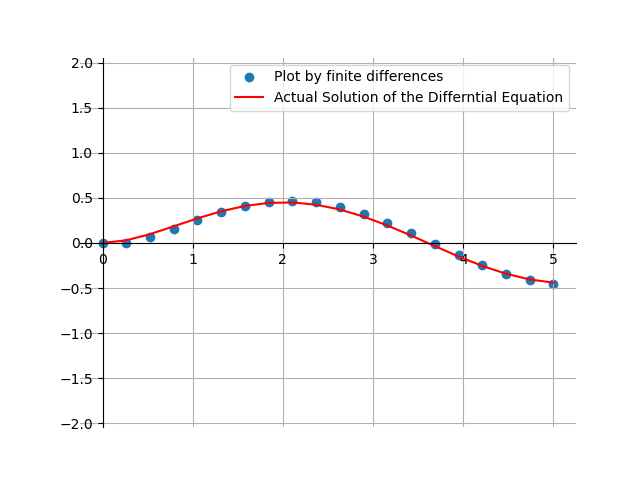
\includegraphics[width=\columnwidth]{figs/fig1.png}  
        \caption{Verification}
        % \columnwidth
    \end{figure}


\end{enumerate}

\end{document}